% ~ 12 pages
\chapter{Identification of Hadronic Tau Lepton Decays using Neural Networks}
\label{sec:rnn}

This chapter investigates the application of neural networks for tau
identification. First it is shown that a multi-layer perceptron (MLP) can
achieve a classification performance comparable to the optimised BDT from the
previous chapter. Subsequently, novel sequence learning techniques are employed
to create classifiers operating on sequences of reconstructed objects. For this
recurrent neural networks based on the LSTM architecture are used on sequences
of tracks in the ID and clusters of energy in the calorimeter system. In this
context, a tau identification algorithm using purely calorimetric information is
developed and a potential application for reducing the trigger rate of a ditau
trigger at the High Luminosity LHC (HL-LHC) is presented. Finally, a model
combining the multi-layer perceptron and the recurrent networks operating on
track and cluster information is developed.

\section{Identification using Feedforward Neural Networks}
\label{sec:ffnn_id}

Before proceeding to sequence classification techniques, the viability of neural
networks to perform tau identification using simple network architectures is
shown. This aids as an introduction to important concepts when training neural
networks. Moreover, the resulting network is used as a building block in the
final model.

The optimised BDT from Chapter~\ref{sec:bdt} is used as a reference for the
investigations in this chapter. Therefore, the models are trained and evaluated
using the same event samples, preselection and reweighting scheme (cf.\
Section~\ref{sec:bdt_eventsim}). In contrast to the hold-out validation used in
the previous chapter, the full event sample is split randomly into training,
validation and testing samples. The samples have a relative size of
\SI{40}{\percent}, \SI{10}{\percent} and \SI{50}{\percent}, respectively. The
purpose of the training and testing samples is the same as before. The
validation sample is monitored during the training process and used to perform
model selection and early stopping of the training. A separate sample, as
opposed to the testing sample, is used to avoid introducing biases in the
performance measurement on the testing sample. This approach is used for the
remainder of this and the following chapter.

To reproduce the performance of the BDT-based tau identification, an MLP with
two hidden layers~(cf.\ Section~\ref{sec:nn_feedforward}) is used. The MLP uses
the same input variables as the optimised BDT. The input variables are
standardised by subtracting the mean and dividing by the standard deviation of
the variable in the training sample. This preprocessing step is important as the
gradient descent algorithm used for training is sensitive to variables on
different scales. The input layer of the MLP consists of 9 (10) neurons
corresponding to the input variables for the 1-prong (3-prong) identification.
Both hidden layers of the MLP have a size of 128 units, which are activated by
rectified linear units (ReLU). A single output neuron is used with the logistic
sigmoid being used as its activation function, therefore returning probabilities
of a \tauhadvis candidate being signal\footnote{Formally the posterior
  probability~$p(\mathcal{S} \mid \mathbf{x})$ of a candidate being
  signal~$\mathcal{S}$ given the input variables~$\mathbf{x}$.}. The binary
cross-entropy loss function is used and minimised by the \textsc{Adam}
optimiser~\cite{adam}. The \textsc{keras} deep learning library~\cite{keras} is
used for building, training and evaluating the model.

In Figure~\ref{fig:roc_mlp_bdt_comparison} the ratio of rejection of the MLP and
the optimised BDT is depicted as a function of the signal efficiency. The
1-prong MLP shows comparable performance above \SI{60}{\percent} signal
efficiency, which approximately corresponds to the tight working point. Over the
intermediate efficiency range the performance is slightly worse. The 3-prong MLP
is consistent with the performance of the optimised BDT identification with a
small improvement at high efficiencies.

\begin{figure}[htb]
  \begin{subfigure}[t]{0.48\textwidth}
    \centering
    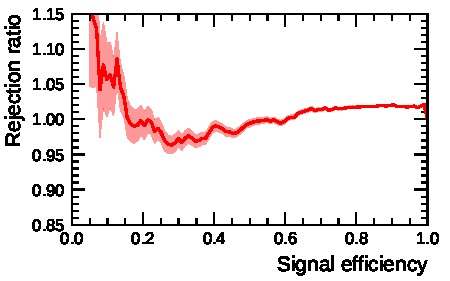
\includegraphics{./figures/rnn/mlp/mlp_bdt_ratio_1p.pdf}
    \subcaption{1-prong}
  \end{subfigure}\hfill
  \begin{subfigure}[t]{0.48\textwidth}
    \centering
    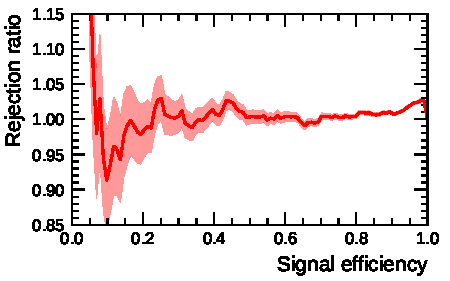
\includegraphics{./figures/rnn/mlp/mlp_bdt_ratio_3p.pdf}
    \subcaption{3-prong}
  \end{subfigure}
  \caption{Ratio of background rejection of the MLP and the optimised BDT as a
    function of signal efficiency. The band indicates the $1\sigma$-interval.}
  \label{fig:roc_mlp_bdt_comparison}
\end{figure}

Overall, both the 1- and 3-prong MLP achieve similar performance characteristics
as the optimised BDT from Chapter~\ref{sec:bdt}, while requiring little
optimisation of model hyperparameters. Therefore, neural networks are shown to
be a viable method of performing tau identification.

\section{Identification using Recurrent Neural Networks}
\label{sec:rnn_id}

Thus far approaches of tau identification use high-level variables that
summarise properties of reconstructed objects in the detector. This has the
advantage that identification can be understood and investigations into
systematic errors are simplified. However, discriminative power can be lost when
transitioning from low- to high-level variables. Therefore an approach is
presented capturing low-level information by employing sequence classification
techniques. A general description of the method is given and subsequently
applied to reconstructed tracks and clusters in the calorimeter.

\subsection{Motivation and General Description}
\label{sec:rnn_descr}

The variable importance of the BDT-based tau identification in
Section~\ref{sec:bdt_var_importance} shows that a large fraction of background
rejection can be attributed to variables derived from tracking information.
Examples are the variables sensitive to the decay length of the tau lepton,
$|S_\text{leadtrack}|$ and~$S_\text{T}^\text{flight}$, as well
as~$f_\text{iso}^\text{track}$ and~$m_\text{track}$. Moreover, during the
preparation of the tau identification for the ATLAS reconstruction release to be
used for the remainder of Run 2, it was observed that \emph{isolation} tracks
offer discriminative power against \tauhadvis candidates from quark- and
gluon-initiated jets. However, migrations between the \emph{isolation} track and
\emph{fake} track categories lead to the necessity to decouple tau
identification from the \emph{isolation} and \emph{fake} tracks by introducing
the \emph{modified isolation} category (cf.\
Section~\ref{sec:reco_track_sel_classif}). This lead to an average rejection
loss of the order of \SI{20}{\percent} for the 1-prong identification, while the
3-prong identification was not significantly affected. Therefore, the aim is to
improve the use of isolation information in reconstructed tracks of \tauhadvis
candidates.

For this purpose recurrent neural networks using the LSTM architecture are used
to classify a sequence of objects reconstructed in the detector. The following
focuses on describing the method utilising tracks in the ID but the use of other
physics objects is analogous. Figure~\ref{fig:track_rnn_schematic} describes the
architecture employed in this chapter. Reconstructed \tauhadvis have a number of
associated tracks, which can be interpreted as elements in a sequence. Each
track in the sequence has variables related to its properties, e.g.\ its
transverse momentum. Moreover, the elements can also be assigned global
information about the \tauhadvis candidate like its visible transverse momentum.
The sequence of tracks is sorted according to a well-defined and physically
motivated ordering scheme. For the RNN using track information a
descending~$p_\text{T}^\text{track}$ ordering is used. \todo{Why this ordering?}
In practice the maximum sequence length is limited by truncation.

\begin{figure}[htb]
  \centering
  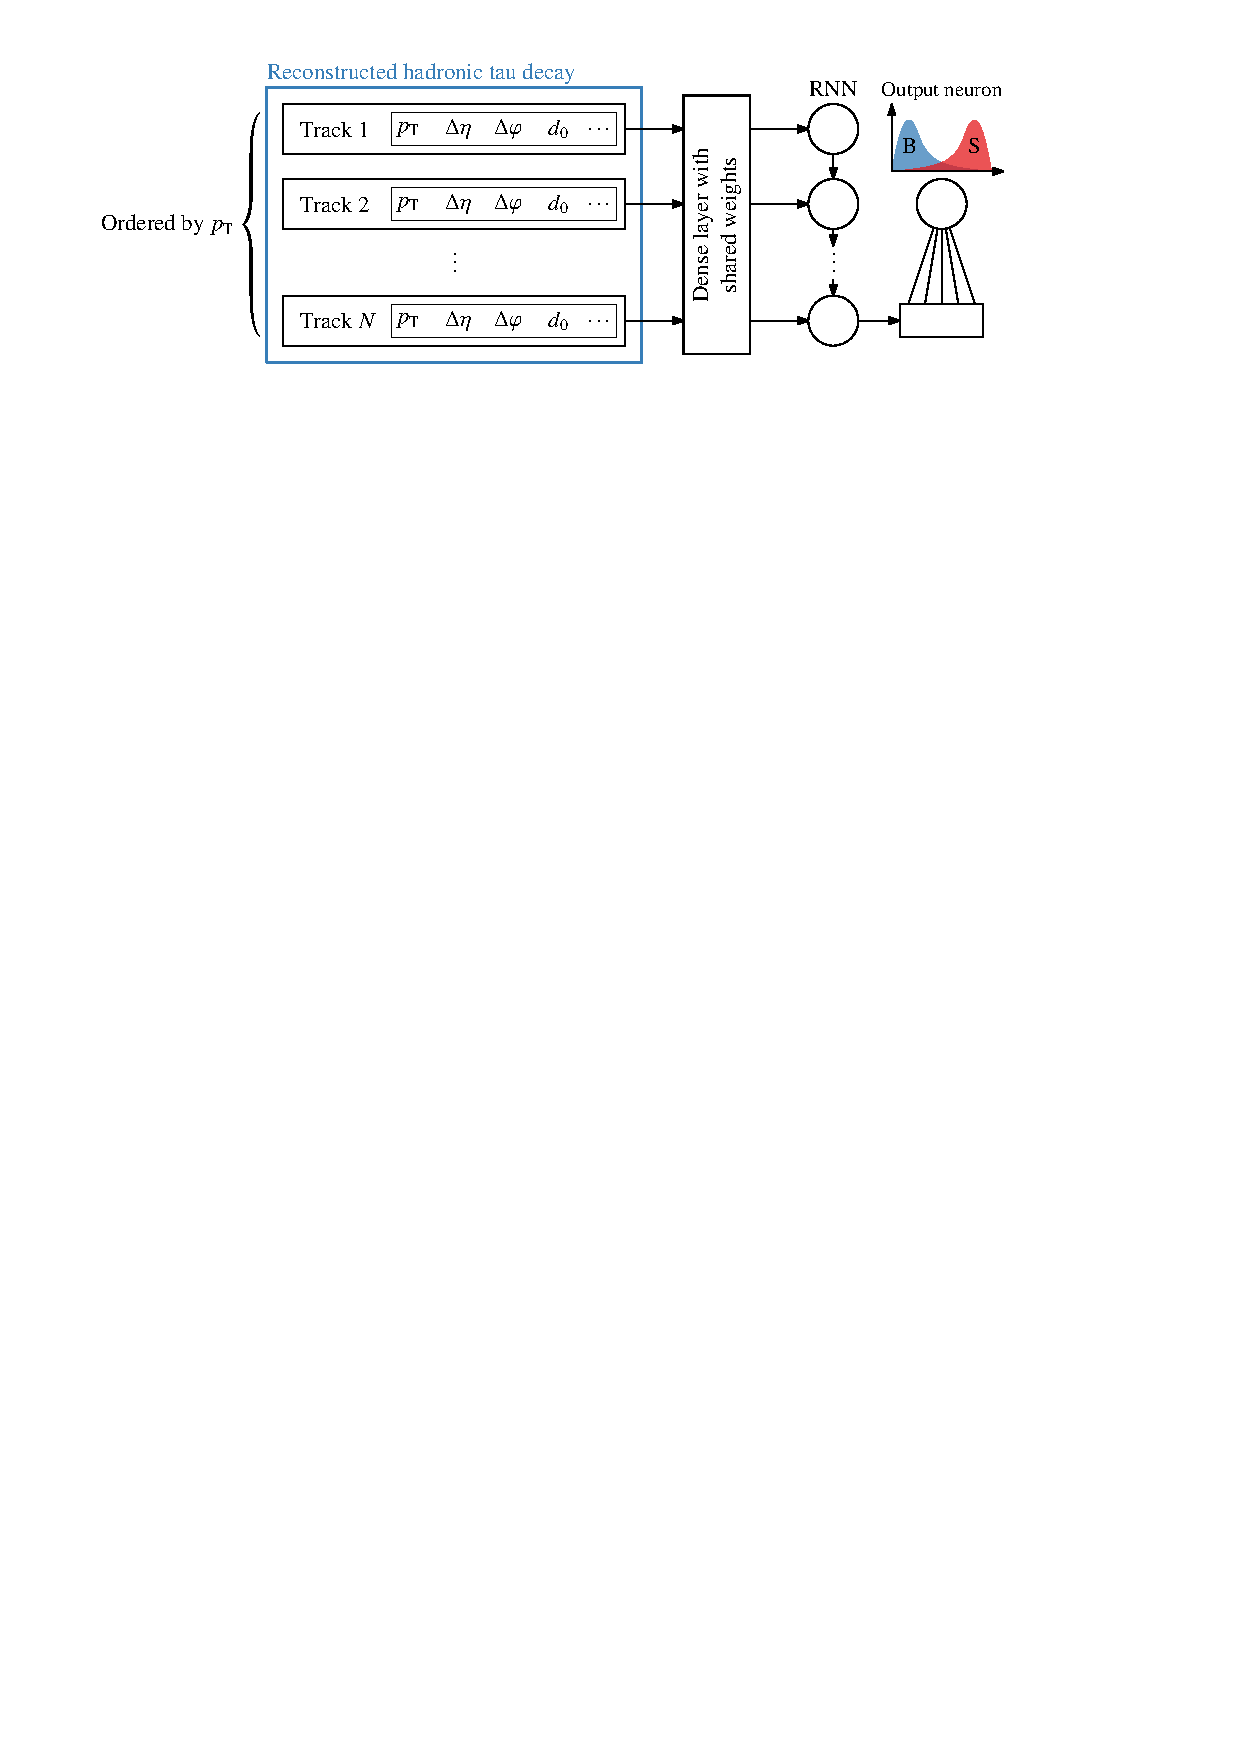
\includegraphics[scale=0.9]{./figures/rnn/track_rnn_schematic.pdf}
  \caption{Schematic description of a recurrent neural network using individual
    tracks for tau identification.}
  \label{fig:track_rnn_schematic}
\end{figure}

The tracks are passed in the predefined order to a dense layer with shared
weights. This layer applies a transformation on the input variables of each
individual track, where the trainable parameters of this transformation are
shared between each element in the sequence. It creates a sequence of
intermediate track representations, which are then passed to the recurrent layer
employing the LSTM architecture. The output of the final time step of the RNN,
consisting of a vector of activations, is passed to a dense layer with one
neuron and logistic sigmoid activation. The activation of the output neuron can
then be used to classify the \tauhadvis candidate as signal or background. The
intermediate layers use the hyperbolic tangent activation function.

\subsection{Network using Reconstructed Tracks in the Inner Detector}
\label{sec:rnn_tracks}

The implementation of the RNN employing track information, hereafter abbreviated
as Track--RNN, uses tracks associated with a \tauhadvis, which are tracks in
the~$\Delta R < 0.4$ cone with respect to the tau axis passing a transverse
momentum threshold of \SI{400}{\MeV} from track reconstruction. The variables
attached to each track are summarised in the following:
\begin{description}
\item[Transverse momentum of track and jet] The transverse momentum of the
  track, $p_\text{T}^\text{track}$, as measured in the tracking system is used.
  The inclusion of the track momentum is crucial as it allows the network to
  discriminate between tracks originating from the hard scattering and soft
  processes. Additionally, the transverse momentum of the anti-$k_t$ jet used to
  seed the \tauhadvis candidate, $p_\text{T}^\text{jet}$, is included in the
  input variables of each track. This allows tracks to be processed differently
  depending on the transverse momentum of the jet seed.

\item[Impact parameters] Information on the impact parameters of the track with
  respect to the associated tau vertex (cf.\
  Section~\ref{sec:reco_vertex_assoc}) is included. The transverse impact
  parameter, $d_0$, is used directly, while the longitudinal impact parameter is
  included as~$z_0 \sin\theta$, where~$\theta$ is the polar angle of the track
  parametrisation.
  % This form accounts for larger errors of~$z_0$ for tracks in the forward
  % region.
  Impact parameter information is important to determine whether a given track
  originated from the tau production vertex. It allows to discriminate between
  tracks from the \tauhad or quark-/gluon-initiated jets and tracks from other
  interactions during the same bunch crossing.

\item[Angular distance to the tau axis] The signed angular distance of the track
  to the tau axis in the transverse~$\Delta \varphi$ and longitudinal
  direction~$\Delta \eta \coloneqq \eta_\text{track} - \eta_\tau$. The transverse
  angular distance~$\Delta \varphi$ is defined analogously to the longitudinal
  case but also accounting for the periodicity in the azimuthal angle~$\varphi$.
  The angular distances allow probing the spacial isolation of the tracks in a
  \tauhadvis candidate.

\item[Track quality criteria] The Track--RNN includes basic track quality
  criteria to allow to reject tracks of low reconstruction quality. For this,
  the number of hits in the pixel layers~$N_\text{pixel}$ and semiconductor
  tracker~$N_\text{SCT}$ are used.
  % IBL TOO!

\item[Electron probability] The probability of the track originating from an
  electron estimated by a likelihood-based discriminant using high-threshold hit
  information in the TRT, $p_\text{HT}$. It is used to identify tracks
  originating from electrons, which may be created in photon conversions.
\end{description}
Including the track category from the multivariate track classification is also
investigated, leading to a small improvement in discrimination power. It is not
included to keep the tau identification largely independent of the multivariate
track classification.

Basic transformations are applied to the input variables to make them suitable
for use in neural networks. Therefore, a logarithm is applied to transverse
momenta~$p_\text{T}^\text{track}$, $p_\text{T}^\text{jet}$ and to the absolute
values of the impact parameters. Similar to the MLP, the input variables have to
be standardised. For transverse momenta and impact parameters this is done by
subtracting an offset and dividing by a scale factor. The offset is the mean of
the corresponding quantity in tracks of the training sample and the scale factor
the standard deviation. Signed angular distances are scaled into the
$[-1, 1]$-interval and similarly the number of hits in the ID into~$[0, 1]$. The
training process is analogous the MLP.

The layer sizes in the architecture depicted in
Figure~\ref{fig:track_rnn_schematic} are optimised by observing the validation
loss while varying the number of units in different layers. A configuration
using 32 units in the shared dense layer and 32 units in the LSTM layer shows
good classification performance, while still being trainable in a moderate
amount of time. Alternative architectures using bidirectional LSTM and multiple
consecutive LSTM layers were investigated and show only marginal improvements
over the simpler model.

In Figure~\ref{fig:ntracks_tau} the number of tracks associated to a given
\tauhadvis candidate is depicted. The number of associated tracks can be large,
especially for background candidates. For practical purposes, the sequence of
tracks is truncated to reduce the memory footprint as well as training and
evaluation time of the network \todo{modelling?}. As the tracks are sorted using
a descending $p_\text{T}^\text{track}$-ordering, truncation will only discard
low momentum tracks. Figure~\ref{fig:ntracks_loss} shows the validation loss for
different numbers of tracks used in the model. The first six tracks show a
significant decrease in validation loss, therefore improving the discriminative
power of the model. Hardly any further improvement is observed after ten tracks.
Therefore, the model only uses the ten leading tracks
in~$p_\text{T}^\text{track}$.

\begin{figure}[htb]
  \begin{subfigure}[t]{0.48\textwidth}
    \centering
    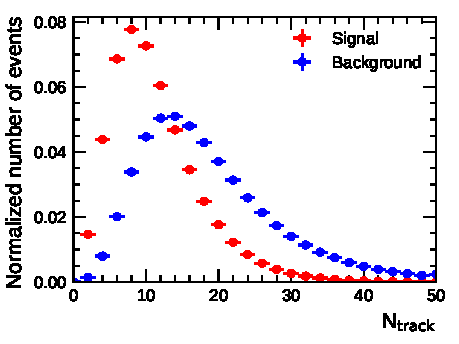
\includegraphics{./figures/rnn/ntrk_1p.pdf}
    \subcaption{Number of tracks associated to a reconstructed 1-prong tau
      candidate.}
    \label{fig:ntracks_tau}
  \end{subfigure}\hfill
  \begin{subfigure}[t]{0.48\textwidth}
    \centering 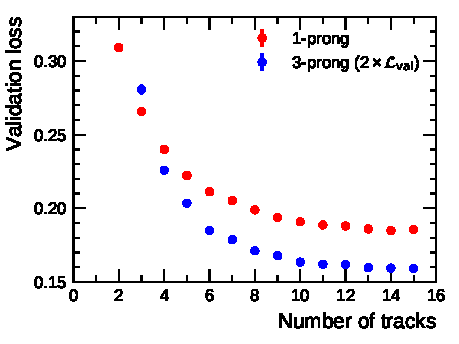
\includegraphics{./figures/rnn/nscan/track_1p_3p.pdf}
    \subcaption{Validation loss (binary cross-entropy) as a function of the
      number of tracks used in the model.}
    \label{fig:ntracks_loss}
  \end{subfigure}
  \caption{Number of tracks associated to a \tauhadvis candidate and their
    impact on the discriminative power of the Track--RNN.}
  \label{fig:rnn_ntracks}
\end{figure}

A comparison of the ROC-curves for the BDT- and RNN-based tau identification is
depicted in Figure~\ref{fig:track_rnn_roc_ratios}. Both the 1- and 3-prong
Track--RNN show performances similar to the optimised BDTs, despite using only
tracking information and~$p_\text{T}^\text{jet}$. The 1-prong Track--RNN shows a
small improvement in rejection of \num{10} to \SI{20}{\percent} over the BDT
depending on the signal efficiency. In contrast to this the 3-prong RNN cannot
exceed the performance of the optimised BDT, only capturing \num{80} to
\SI{90}{\percent} of rejection. These results indicate that the available
information in tracks is not fully exploited in the current BDT-based
identification.

\begin{figure}[htb]
  \begin{subfigure}[t]{0.48\textwidth}
    \centering
    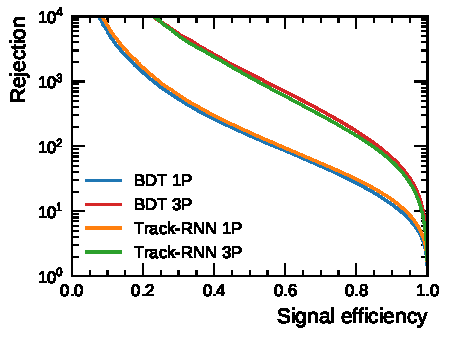
\includegraphics{./figures/rnn/track/roc.pdf}
    \subcaption{ROC-curves for 1-prong (1P) and 3-prong (3P) tau
      identification.}
  \end{subfigure}\hfill
  \begin{subfigure}[t]{0.48\textwidth}
    \centering
    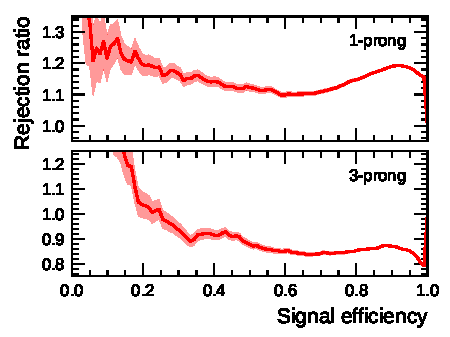
\includegraphics{./figures/rnn/track/ratios.pdf}
    \subcaption{Ratio of rejection of the Track--RNN and the optimised BDT. The
      band indicates the $1\sigma$-interval.}
  \end{subfigure}
  \caption{Classification performance of the Track--RNN compared to the
    optimised BDT for tau identification.}
  \label{fig:track_rnn_roc_ratios}
\end{figure}

Due to the complexity of the network, interpretation of the model based on the
weights learned during training is not possible. It must be viewed as a black
box where only the input and the output can be accessed. Nevertheless, the
variable importance and linear correlations of output and inputs can be
evaluated to gain a better understanding of the model. In
Table~\ref{tab:var_importance_track_rnn} the importance of the input variables
is estimated by removing groups of related variables and retraining the model.
The increase in validation loss is used to rank the importance of each group.
The table shows that the impact parameters and transverse momenta have a large
impact on the validation loss. They are essential to identify tracks originating
from the associated primary vertex as opposed to tracks from other hard
interactions or pile-up. The angular distances~$\Delta \eta$
and~$\Delta \varphi$ show an importance similar to the transverse momenta.
Compared to tracks in \tauhadvis candidates created by quark- or gluon-initiated
jets, tracks from hadronic tau decays are expected to be close to the tau axis
resulting in small angular distances. The number of hits in the ID
and~$p_\text{HT}$ show only a small importance in the Track--RNN, with
$p_\text{HT}$ being a candidate for removal.

\begin{table}[htb]
  \centering
  {\small\begin{tabular}{p{5cm}S[table-format=1.4(4)]S[retain-explicit-plus, table-format=+2.1]}
  \toprule
  {Variables} & {Validation loss} & {Loss increase} \\
  \midrule
  \parbox[c]{\hsize}{Impact parameter \newline $d_0$, $z_0 \sin\theta$}
          & 0.2831 +- 0.0005 & + 48.4 \,\si{\percent} \\[1.2em]
  \parbox[c]{\hsize}{Transverse momentum \newline $p_\text{T}^\text{track}$, $p_\text{T}^\text{jet}$}
          & 0.2410 +- 0.0007 & + 26.3 \,\si{\percent} \\[1.2em]
  \parbox[c]{\hsize}{Angular distance \newline $\Delta \eta$, $\Delta \varphi$}
          & 0.2304 +- 0.0003 & + 20.8 \,\si{\percent} \\[1.2em]
  \parbox[c]{\hsize}{Hits in ID \newline $N_\text{hit}^\text{pixel}$, $N_\text{hit}^\text{SCT}$}
          & 0.2036 +- 0.0013 & + 6.7 \,\si{\percent} \\[1.2em]
  \parbox[c]{\hsize}{Electron probability (TRT) \newline $p_\text{HT}$}
          & 0.1930 +- 0.0004 & + 1.2 \,\si{\percent}\\
  \bottomrule
\end{tabular}

%%% Local Variables:
%%% mode: latex
%%% TeX-master: "../mythesis"
%%% End:
}
  \caption{Variable importance of the 1-prong Track--RNN estimated by the
    increase in validation loss when removing groups of input variables.}
  \label{tab:var_importance_track_rnn}
\end{table}

In Figure~\ref{fig:track_rnn_correlations} the linear correlation coefficients
between the input variables of each track in the sequence and the signal
probability estimate~$p_\text{RNN}$ of the Track--RNN are depicted. In real
\tauhadvis the leading tracks in transverse momentum typically correspond to the
charged pions of the tau decay. This results in a change in sign of the
correlation coefficient after the first (first three) track(s) for 1-prong
(3-prong) candidates. The correlation of~$p_\text{T}^\text{track}$
% in Figure~\ref{fig:track_rnn_corr_pt}
is positive for the leading tracks. Therefore, \tauhadvis candidates with
leading tracks of high transverse momentum are more likely to have larger signal
probabilities according to the model. In contrast to this, subleading tracks
with large transverse momentum tend to reduce the signal probability, thus are
more likely associated with background \tauhadvis candidates. Similarly, the
correlation of~$|z_0 \sin\theta|$ with the output
% in Figure~\ref{fig:track_rnn_corr_z0}
shows that signal candidates are more likely to have leading tracks close to the
associated primary vertex, while subleading tracks exhibit larger distances. The
same behaviour is observed for~$|d_0|$ and the $\Delta R$-distance of tracks to
the tau axis (cf.\ Appendix~\ref{app:corr_dr}), which is related to the signed
angular distances~$\Delta \eta$ and~$\Delta \varphi$ included in the model.
% Figure~\ref{fig:track_rnn_corr_z0} shows that signal candidates are more likely
% to have leading tracks close to the primary vertex, while subleading tracks
% exhibit larger distances to the vertex. The same behaviour is observed for the
% transverse impact parameter~$|d_0|$ and the $\Delta R$-distance to the tau axis,
% which can be calculated using the signed angular distances~$\Delta \eta$ and
% $\Delta \varphi$.

\begin{figure}[htb]
  \centering
  \begin{subfigure}[t]{0.48\textwidth}
    \centering
    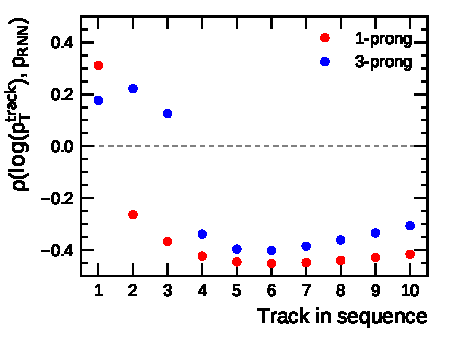
\includegraphics{./figures/rnn/track/pt_corr.pdf}
    \subcaption{Transverse momentum of the track~$p_\text{T}^\text{track}$.}
    \label{fig:track_rnn_corr_pt}
  \end{subfigure}\hfill
  \begin{subfigure}[t]{0.48\textwidth}
    \centering
    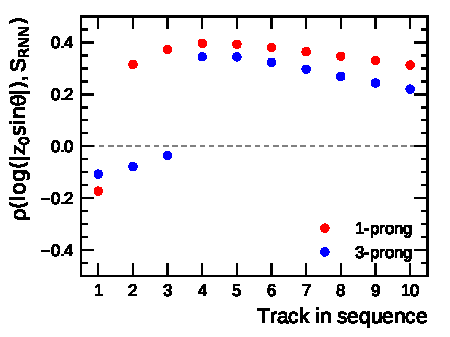
\includegraphics{./figures/rnn/track/z0_corr.pdf}
    \subcaption{Longitudinal impact parameter with respect to the tau primary
      vertex~$|z_0 \sin\theta|$.}
    \label{fig:track_rnn_corr_z0}
  \end{subfigure}
  \caption{Linear correlation coefficient between input variables and signal
    probability~$p_\text{RNN}$ estimated by the model. The coefficient is
    determined on the testing sample combining signal and background candidates
    with equal total weight.}
  \label{fig:track_rnn_correlations}
\end{figure}

By using impact parameters to identify tracks originating from the tau primary
vertex, information on the expected transverse momentum distribution for
individual tracks of a \tauhadvis and requiring spacial isolation, the
Track--RNN performs comparably to the BDT-based identification. A detailed
evaluation of the background rejection for the identification working points is
given at a later point.

\subsection{Network using Clusters in the Calorimeter System}
\label{sec:rnn_clusters}

The BDT-based tau identification makes extensive use of calorimetric information
by using clusters of calorimeter cells created by the TopoCluster algorithm and
quantities directly calculated from individual cells. Therefore, a separate
recurrent network is developed employing TopoClusters associated with the jet
seeding a \tauhadvis candidate, hereafter called the Cluster--RNN. The variable
selection is given in the following:
\begin{description}
\item[Transverse energy/momentum] The transverse energy of the cluster,
  $E_\text{T}$, and the transverse momentum of the jet seeding the \tauhadvis
  candidate, $p_\text{T}^\text{jet}$, are used. The motivation for including
  these variables is analogous to the Track--RNN.

\item[Angular distance to the tau axis] The signed angular distance of the
  cluster barycentre to the tau axis in the longitudinal~$\Delta \eta$ and
  transverse plane~$\Delta \varphi$.

\item[Cluster and signal moments] Identification variables like the central
  energy fraction, $f_\text{cent}$, use quantities calculated from individual
  cells in the calorimeter. Cell-level information is not available in the
  samples used for this study. Therefore, cluster and signal moments of
  TopoClusters are used to obtain information on cluster shape and energy
  density.

  The moments used for the Cluster--RNN are summarised in the following. The
  lateral shower width, $\langle R^2 \rangle$, given by the second moment of the
  radial distance~$R$ between cluster cells and shower axis; the longitudinal
  shower width, $\langle \lambda^2 \rangle$, with the distance~$\lambda$ of
  cells from the barycentre of shower energy measured along the shower axis; the
  mean energy density, $\langle \rho \rangle$; the energy fraction of the most
  energetic cell, $f_\text{max}$; and the depth of the shower centre,
  $\lambda_\text{centre}$, measured from the face of the
  calorimeter\footnote{While $\lambda_\text{centre}$ itself is not a cluster
    moment, it is derived from the first moments of the cartesian cell
    coordinates.} are used. These cluster and signal moments are calculated by
  the TopoCluster algorithm~\cite{atlas_topoclustering}.
\end{description}
Additionally, energy fractions of clusters in the individual samplings of the
electromagnetic calorimeter and the probability of a cluster to originate from
an electromagnetic
shower~$\mathcal{P}_\text{clus}^\text{EM}$~\cite{atlas_topoclustering}, which is
used in the local hadronic calibration, are investigated. These variables are
not found to improve the classification power of the cluster-based
identification.

The input variables are transformed and standardised similar to the track-based
identification. The cluster moments are log-transformed and standardised by
subtracting an offset and dividing by a scale factor. The signal
moment~$f_\text{max}$ does not require preprocessing. The remaining variables
are processed in analogy to the Track--RNN.

The architecture used for the Cluster--RNN is identical to the one used for the
Track-RNN. However, the number of units in the LSTM layer is reduced to 24 (from
32), while the shared dense layer remains at 32 units. Clusters are passed in
descending~$E_\text{T}$-ordering to the network. Figure~\ref{fig:rnn_nclusters}
shows the number of clusters in the jet used to seed the \tauhadvis candidate
and the impact of truncating the cluster sequence on the validation loss. The
cluster-based identification shows little improvement in classification power
after the six leading clusters in~$E_\text{T}$. Therefore, the input sequence
passed to the model is truncated after six clusters.

\begin{figure}[htb]
  \begin{subfigure}[t]{0.48\textwidth}
    \centering
    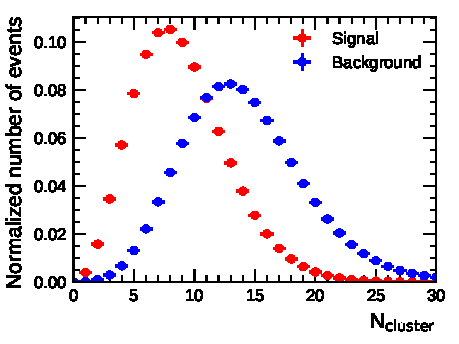
\includegraphics{./figures/rnn/ncls_1p.pdf}
    \subcaption{Number of clusters in the anti-$k_t$ jet used to seed the
      1-prong \tauhadvis candidates.}
  \end{subfigure}\hfill
  \begin{subfigure}[t]{0.48\textwidth}
    \centering
    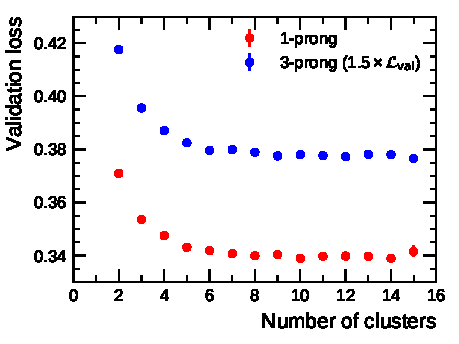
\includegraphics{./figures/rnn/nscan/cluster_1p_3p.pdf}
    \subcaption{Validation loss as a function of the number of clusters used in
      the model.}
  \end{subfigure}
  \caption{Number of clusters associated to a \tauhadvis candidate and their
    impact on the discriminative power of the Cluster--RNN.}
  \label{fig:rnn_nclusters}
\end{figure}

The classification performance after training the model for 1- and 3-prong
\tauhadvis candidates separately is shown in
Figure~\ref{fig:cluster_rnn_roc_ratios}. The 1- and 3-prong Cluster--RNN show
similar performance characteristics. However, the purely cluster-based
identification cannot reach performances comparable to the tau identification
using the optimised BDT. For the identification of 1-prong \tauhadvis a fraction
of \num{10} to \SI{40}{\percent} of rejection is reached, depending on the
signal efficiency. Due to the large rejection of the 3-prong BDT-based
identification and the missing track information, the rejection of the
Cluster--RNN can only reach a fraction of \num{2} to \SI{10}{\percent} of the of
the BDT performance.

\begin{figure}[htb]
  \begin{subfigure}[t]{0.48\textwidth}
    \centering
    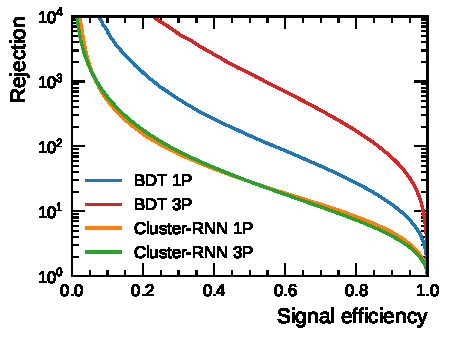
\includegraphics{./figures/rnn/cluster/roc.pdf}
    \subcaption{ROC-curves for 1-prong (1P) and 3-prong (3P) tau
      identification.}
  \end{subfigure}\hfill
  \begin{subfigure}[t]{0.48\textwidth}
    \centering
    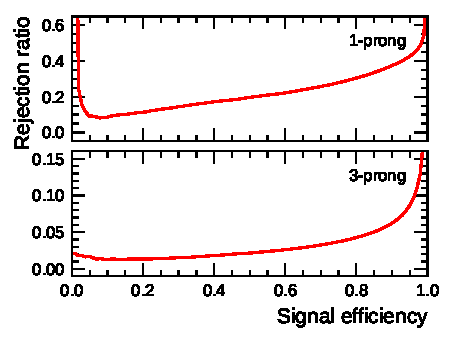
\includegraphics{./figures/rnn/cluster/ratios.pdf}
    \subcaption{Ratio of rejection of the Cluster--RNN and the optimised BDT.}
  \end{subfigure}
  \caption{Classification performance of the Cluster--RNN compared to the
    optimised BDT for tau identification.}
  \label{fig:cluster_rnn_roc_ratios}
\end{figure}

The most important variables for the operation of the Cluster--RNN are the
angular distances~$\Delta \eta$ and~$\Delta \varphi$ followed by the
$E_\text{T}$ of the cluster and the transverse momentum of the jet
seed~$p_\text{T}^\text{jet}$. The cluster and signal moments, while still
contributing significantly to the discriminative power, are the least important.
This variable ranking indicates that a significant part of the discriminative
power is obtained by requiring isolated showers close to the tau axis.

Due to the small background rejection, the standalone operation of the
Cluster--RNN is not of interest to the offline reconstruction of \tauhadvis.
However, it can potentially be used for tau identification at trigger-level,
where track and vertex reconstruction are infeasible due to time constraints.

\subsubsection{Online Ditau Identification at the High Luminosity LHC}
\label{sec:hlt_rate_reduction}

The Phase-II upgrade of the LHC called the High Luminosity LHC (HL-LHC) is
foreseen to be finished by 2026. It will increase the instantaneous luminosity
to~\num{5}\,--\,\SI{7.5e34}{\per\square\centi\metre\per\second} at a
centre-of-mass energy
of~$\sqrt{s} = \SI{14}{\TeV}$~\cite{hl_lhc_prelim_design_report}. This
corresponds to a five- to sevenfold increase in luminosity with respect to the
beginning of Run~2 and increases the average number of interactions per bunch
crossing to up to \num{200}. The increase in particle density poses a challenge
to the trigger and reconstruction algorithms.

An upgrade of the ATLAS trigger with a \emph{Global Trigger System} aims to
provide access to the full calorimeter granularity with topoclustering and jet
finding using iterative jet algorithms in regions of
interest~\cite{phase_2_scoping}. This aims to improve the identification of
physics objects at trigger-level to cope with increasing trigger rates due to
pile-up and other background processes. Due to the availability of full
calorimeter granularity, offline reconstructed \tauhadvis can be used to give
prospects of the potential performance of triggers for \tauhadvis in the HL-LHC
environment.

A prospective study focusing on the usage of the cluster-based RNN for
identification of \tauhadvis in a ditau trigger is given. Offline \tauhadvis are
used as an approximation to reconstructed taus at trigger-level after the
Phase-II upgrade. The study uses simulated samples
of~$Z / \gamma^* \to \tau \tau$ and dijets at HL-LHC conditions with
centre-of-mass energy~$\sqrt{s}=\SI{14}{\TeV}$ and average interactions per
bunch crossing~$\mu = 200$ (cf.\ Appendix~\ref{app:upgrade_samples}).

The cluster-based RNN identification is retrained on \tauhadvis candidates of
the HL-LHC upgrade samples using the same preselection used for the BDT
identification in Chapter~\ref{sec:bdt} with the exception of any
tracking-related requirements. The leading and subleading \tauhadvis candidates
with respect to the reconstructed transverse momentum (using Run 2 calibrations)
are selected in a given event, while additionally requiring two truth-matched
hadronic tau decays for the signal sample. The RNN identification is applied to
each \tauhadvis candidate individually resulting in two identification scores
per event. The leading and subleading \tauhadvis~$p_\text{T}$ and identification
scores are combined in a logistic regression to assign a single ditau
identification score to each event.

The \SI{200}{\kilo\hertz} accept rate of the subsequent trigger
level~\cite{phase_2_scoping} limits the maximum rate of the ditau trigger.
Achieving this rate requires $p_\text{T}$-thresholds on leading and subleading
\tauhadvis as well as application of the ditau identification. The thresholds
should be kept low to ensure high signal acceptance for physics analyses. For
the purposes of this study a fixed cut on the identification score \todo{plot
  with cut?} is used to identify ditau events.

Due to the large dijet production cross section, it is assumed that the dijet
events in the simulated sample correspond to a trigger rate equal to the average
bunch crossing rate of~\SI{31.6}{\mega\hertz}. In
Figure~\ref{fig:rate_vs_thresholds} the trigger rate is shown as a function of
the leading and subleading \tauhadvis $p_\text{T}$-thresholds after applying
ditau identification. The target rate can be achieved with an offline
$p_\text{T}$-threshold of \SI{25}{\GeV} on both \tauhadvis candidates. As a
comparison, the primary ditau triggers used for the 2016 $pp$ data taking period
used thresholds of \SI{35}{\GeV} and \SI{25}{\GeV}~\cite{tautrigger_run2}.
Figure~\ref{fig:ditau_trigger_eff} \todo{rather plot subleading?} shows the
efficiency of the identification using the specified thresholds with respect to
events containing truth-matched \tauhadvis pairs. The ditau efficiency starts to
plateau at true visible transverse momenta
of~$p_\text{T}^\text{true} > \SI{40}{\GeV}$ of the leading \tauhadvis with an
efficiency of approximately~\SI{90}{\percent}.

\begin{figure}[htb]
  \centering
  \begin{subfigure}[t]{0.48\textwidth}
    \centering
    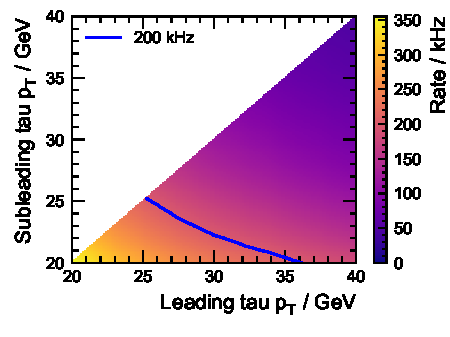
\includegraphics{./figures/rnn/trigger/pt_rate_reg.pdf}
    \subcaption{Trigger rate after RNN-based identification as a function of
      leading and subleading \tauhadvis $p_\text{T}$-threshold.}
    \label{fig:rate_vs_thresholds}
  \end{subfigure}\hfill
  \begin{subfigure}[t]{0.48\textwidth}
    \centering
    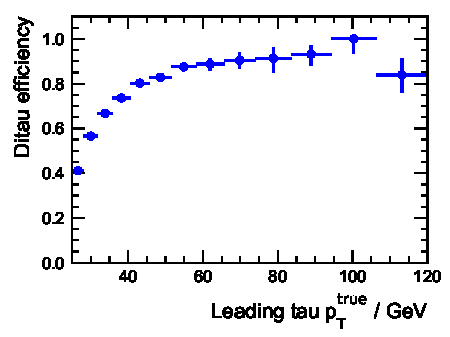
\includegraphics{./figures/rnn/trigger/taueff_reg.pdf}
    \subcaption{Efficiency of the RNN-based identification with \pt-thresholds
      of \SI{25}{\GeV} w.r.t.\ truth-matched \tauhadvis pairs in
      $\text{Z} \to \tau\tau$
      fulfilling~$p_\text{T, vis}^\text{true} > \SI{25}{\GeV}$.}
    \label{fig:ditau_trigger_eff}
  \end{subfigure}
  \caption{Performance of the TopoCluster-based ditau identification for use in
    a ditau trigger at the HL-LHC.}
  \label{fig:rnn_ditau_trigger}
\end{figure}

First scoping studies of the ATLAS upgrade~\cite{phase_2_scoping} conceive a
ditau trigger with offline \tauhadvis \pt-threshold on the leading and
subleading tau of \SI{40}{\GeV} and \SI{30}{\GeV}, respectively. The approach of
using the Cluster--RNN for tau identification achieves the target rate at
reduced \tauhadvis \pt-thresholds of~\SI{25}{\GeV}. The efficiency of the
selection shows opportunities for further enhancements by employing a proper tau
energy calibrations for HL-LHC conditions and using a more advanced decision
threshold for the ditau identification. The decision threshold could be loosened
with increasing transverse momentum to ensure a quicker turn-on and full
efficiency at high-\pt.

\subsection{Combining Recurrent Neural Networks and MLP}
\label{sec:rnn_combined}
After introducing the MLP using high-level identification variables as well as
the track- and cluster-based RNNs, a network combining these models is trained.
Although the models carry redundant information, an improvement in background
rejection can be expected.

The combined model builds on the architectures of the previously developed MLP,
Track-- and Cluster--RNN. A schematic description of the model is given in
Figure~\ref{fig:schematic_combined}. The combined model contains three distinct
branches. The branches using track and cluster inputs are inherited from the
Track-- and Cluster-RNN, respectively. The sizes of the shared dense and LSTM
layers remain unchanged. The third branch is derived from the MLP using
high-level identification variables. While the first two layers are unchanged, a
third dense layer with 16 units is added. The three branches are merged by
concatenating their outputs and subsequently reduced to a single output neuron
in a final dense layer using the logistic sigmoid activation function. The input
variables of each branch are transformed and standardised as given in the
respective section.

\begin{figure}[htb]
  \centering
  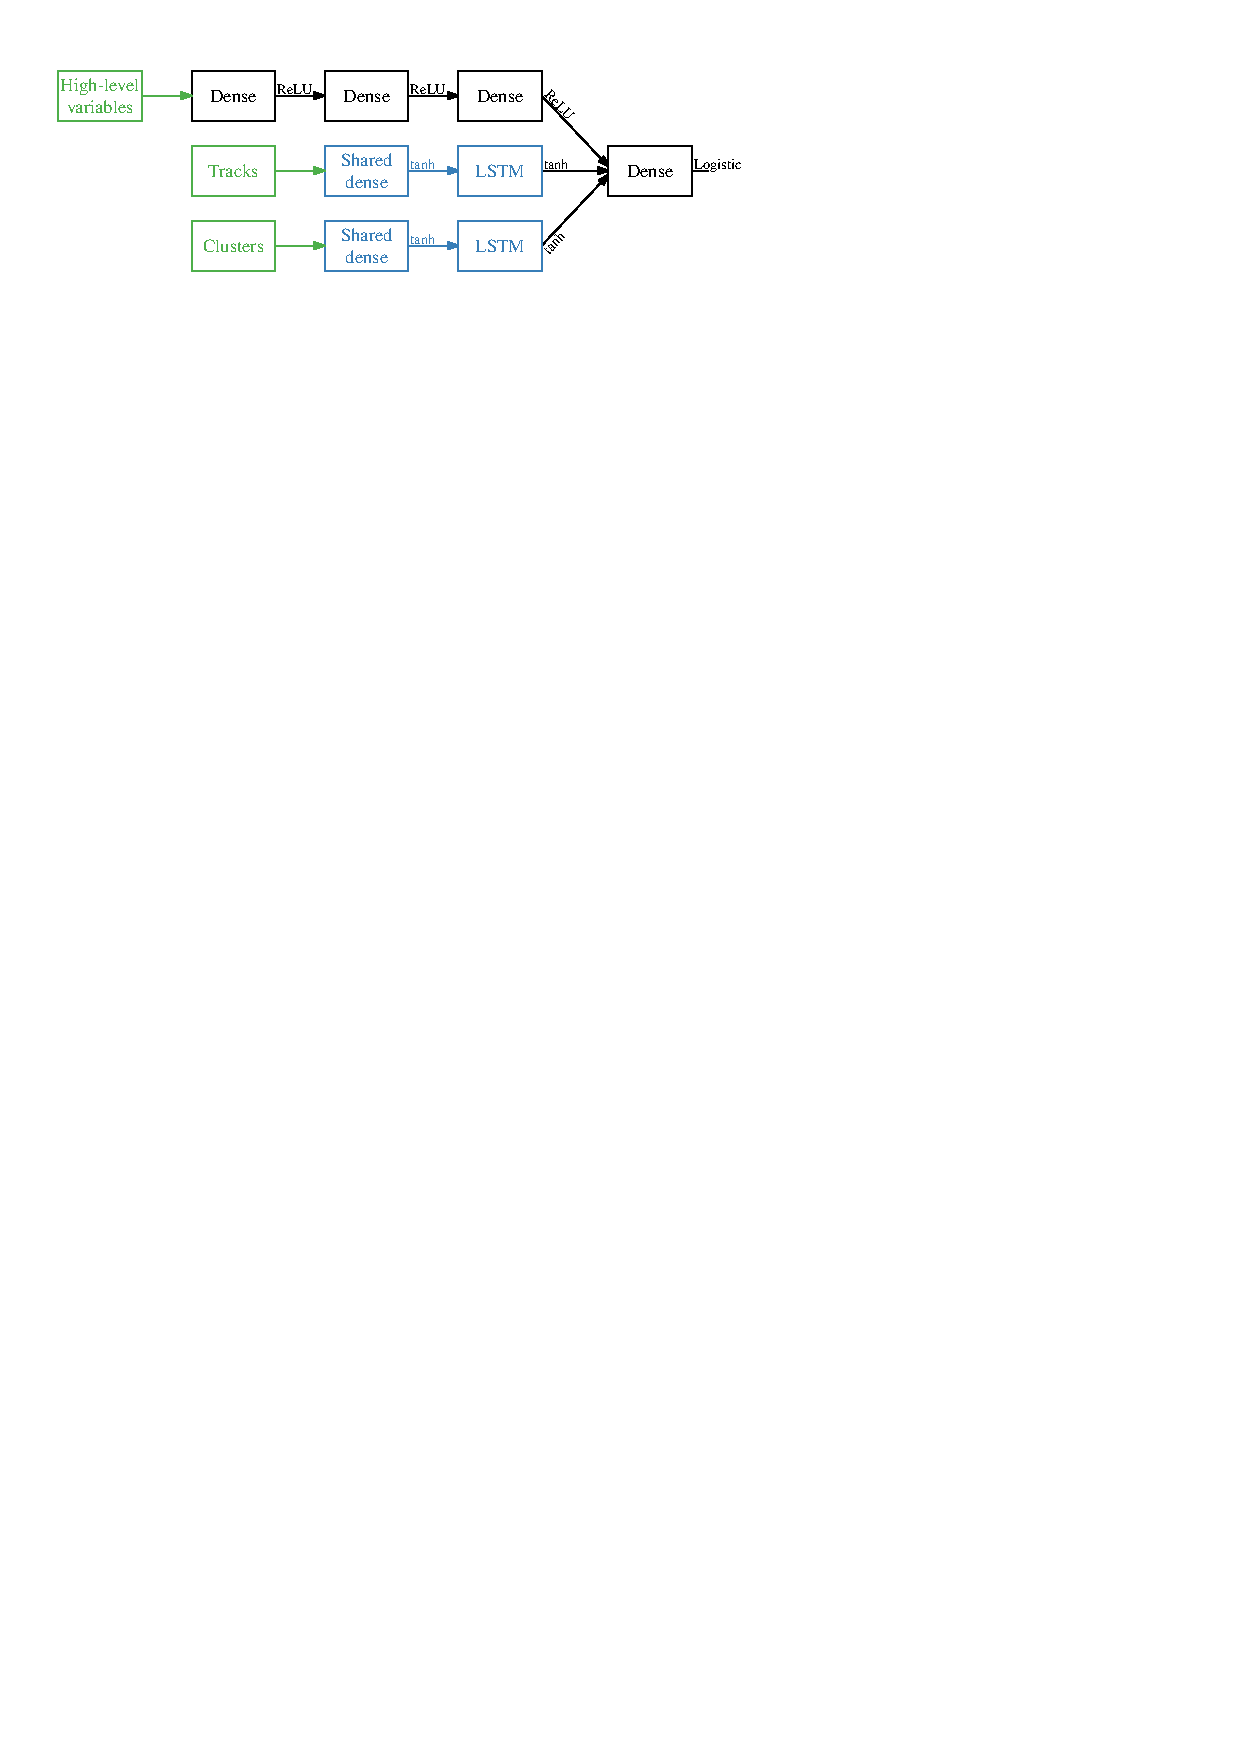
\includegraphics{./figures/rnn/combined_architecture.pdf}
  \caption{Architecture of the combined model operating on high-level
    identification variables and sequences of tracks and clusters. The
    activation function is denoted after each layer (cf.\ Chapter~\ref{sec:ml}).
    Layers operating on sequential inputs are highlighted in blue.}
  \label{fig:schematic_combined}
\end{figure}

Figure~\ref{fig:roc_combined} compares the ROC-curves of the combined model with
the optimised BDTs from Chapter~\ref{sec:bdt}. A model combining MLP and
Track--RNN without including the Cluster--RNN is also shown. The combined model
shows a significant improvement on the BDT-based tau identification. The
background rejection is increased by a factor of two for 1-prong and
approximately \SI{50}{\percent} for 3-prong candidates. The contribution of
cluster information to the rejection is small, with an improvement of
approximately \SI{10}{\percent} in background rejection. Omitting the cluster
branch would allow to simplify the model significantly without incurring a large
loss in discriminative power. \todo{Write sth.\ about Track+Cluster}

\begin{figure}[htb]
  \begin{subfigure}[t]{0.48\textwidth}
    \centering
    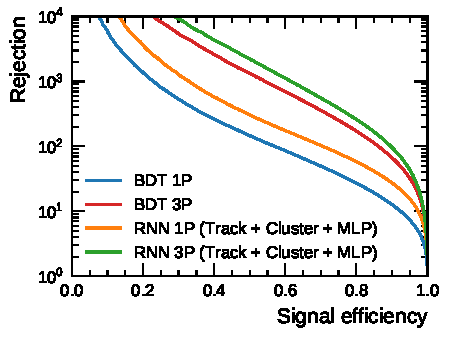
\includegraphics{./figures/rnn/combined/roc.pdf}
    \subcaption{ROC-curves for 1-prong (1P) and 3-prong (3P) tau identification.}
  \end{subfigure}\hfill
  \begin{subfigure}[t]{0.48\textwidth}
    \centering
    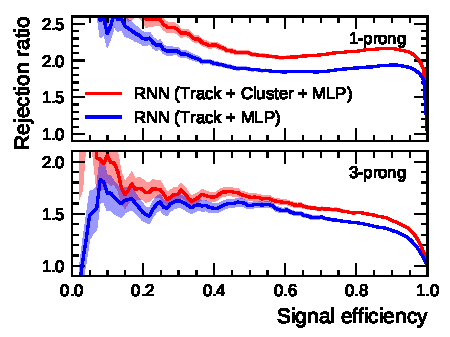
\includegraphics{./figures/rnn/combined/ratios.pdf}
    \subcaption{Ratio of rejection of the combined model and the optimised BDT.}
  \end{subfigure}
  \caption{Classification performance of the combined model compared to the
    optimised BDT for tau identification.}
  \label{fig:roc_combined}
\end{figure}

The \pt-dependence of the background rejection for the 1- and 3-prong tight
working points using the RNN is shown in
Figure~\ref{fig:combined_working_points} and compared with the BDT-based
identification. The combined model shows a relative increase in rejection at the
tight working point ranging from \num{70} to \SI{150}{\percent} for 1-prong and
\num{40} to \SI{100}{\percent} for 3-prong tau identification over the optimised
BDT-based model. In both cases an improvement in background rejection with
increasing \tauhadvis \pt is observed. A possible explanation for this behaviour
is the enhanced use of isolation information in the RNN leading to an improved
background rejection due to the increasing charged-particle multiplicity of
quark- or gluon-initiated jets at high transverse momenta. In contrast to the
RNN, the selection of \tauhadvis with one or three tracks classified as
\emph{charged} is not optimised to reject jet background, therefore allowing the
dedicated algorithm to further improve the classification. The medium and loose
working points show similar improvements (cf.\ Appendix~\ref{app:rnn_wp}).

\begin{figure}[htb]
  \begin{subfigure}[t]{0.48\textwidth}
    \centering
    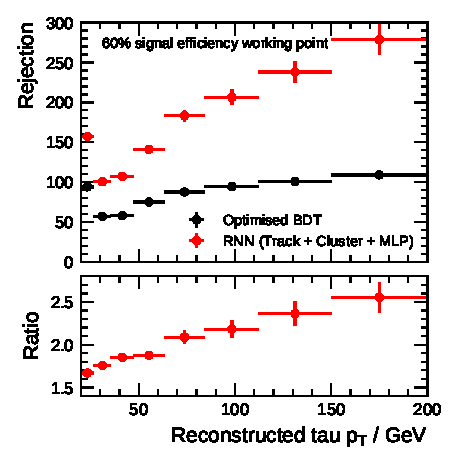
\includegraphics{./figures/rnn/combined/rnn_tight_1p.pdf}
    \subcaption{1-prong}
  \end{subfigure}\hfill
  \begin{subfigure}[t]{0.48\textwidth}
    \centering
    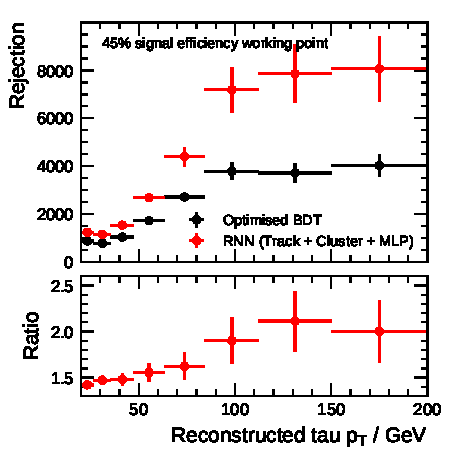
\includegraphics{./figures/rnn/combined/rnn_tight_3p.pdf}
    \subcaption{3-prong}
  \end{subfigure}
  \caption{Background rejection at the tight working point as a function of the
    \tauhadvis $p_\text{T}$ at tau energy scale for the BDT- and RNN-based
    identification.}
  \label{fig:combined_working_points}
\end{figure}

The improved background rejection allows to increase the signal efficiency of
the working points, while still maintaining a rejection comparable to the
nominal working point of the BDT-based identification. An example is the
efficiency of the tight working point for the 1-prong identification, which can
be increased from \num{60} to \SI{70}{\percent}. In doing this the rejection of
fake \tauhadvis candidates with transverse momentum of \SI{20}{\GeV} matches the
rejection of the BDT using the nominal tight working point. For larger
\tauhadvis \pt the rejection of the RNN at the loosened working point still
exceeds the BDT-based identification. Analogously, the signal efficiency of the
3-prong tight working point can be increased from \SI{45}{\percent} to
\SI{50}{\percent}. A comparison is shown in Figure~\ref{fig:loosened_wp}.

Analyses requiring two \tauhadvis with tight identification in the reconstructed
final state, e.g.\ measurements in the~\mbox{$H \to \tauhad \tauhad$} channel,
can benefit from introducing working points with increased signal efficiency.
Assuming the identification scores of the \tauhadvis in the final state are
uncorrelated, a 1-prong working point with \SI{70}{\percent} signal efficiency
increases the number of signal events by \SI{36}{\percent} compared to the
nominal working point. For a 3-prong working point with \SI{50}{\percent} signal
efficiency the signal yield would be increased by \SI{23}{\percent}. The
RNN-based identification can achieve these working point efficiencies, while
offering rejection rates matching or exceeding the nominal working points of the
optimised BDT. For searches of additional heavy neutral Higgs and gauge
bosons~\cite{zprime}, where the reconstructed final state is expected to contain
\tauhadvis with high transverse momenta, the working point efficiencies could be
increased even further.
% 1-prong
% 0.6 * 0.6 = 0.36
% 0.7 * 0.7 = 0.49
% 0.49 / 0.36 = 1.3611111111 -> 36 % relative increase in signal
%
% 3-prong
% 0.45 * 0.45 = 0.2025
% 0.5 * 0.5 = 0.25
% 0.25 / 0.2025 = 1.234567901234568 -> 23 % relative increase in signal

\begin{figure}[htbp]
  \begin{subfigure}[t]{0.48\textwidth}
    \centering
    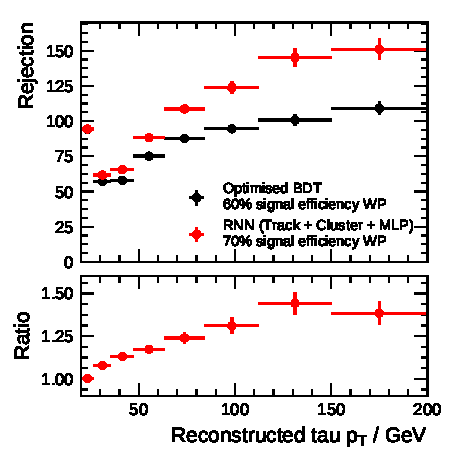
\includegraphics{./figures/rnn/combined/rnn_loosened_tight_1p.pdf}
    \subcaption{1-prong}
  \end{subfigure}\hfill
  \begin{subfigure}[t]{0.48\textwidth}
    \centering
    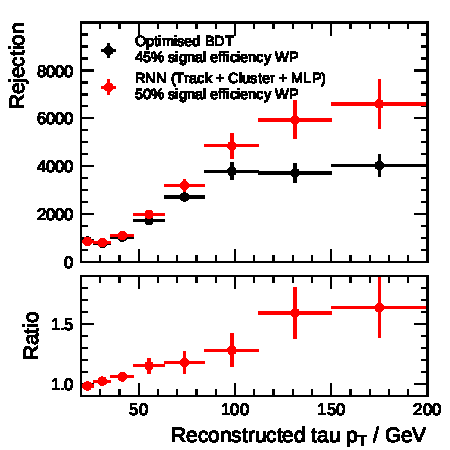
\includegraphics{./figures/rnn/combined/rnn_loosened_tight_3p.pdf}
    \subcaption{3-prong}
  \end{subfigure}
  \caption{Comparison of the background rejection of the RNN-based
    identification at a working point (WP) with increased signal efficiency with
    the nominal tight working point of the BDT.}
  \label{fig:loosened_wp}
\end{figure}

The models developed in this chapter present an novel approach of performing tau
identification. They show a promising performance over the tau identification
strategy currently employed in the ATLAS experiment. Thus far the results are
based on simulated data and still require validation and performance
measurements using collision data taken with the detector.

\todo[inline]{Whats with Track-RNN + Cluster-RNN? Definitely should have that --
  see if we can skip on the high-level info.}

\todo[inline]{Have at least an exemplary RNN score in the appendix.}

\todo[inline]{Missing hits for taus decaying after pixel layers. Questionable
  modelling of impact parameters. Also number of hits is directly used. Should
  not affect low momentum taus. $p_\text{T} = \SI{200}{\GeV}$ taus -- less than
  \SI{5}{\percent} decay after the IBL.}

\todo[inline]{Pile-up dependency of RNN vs BDT-ID}

\todo[inline]{Regained lost rejection from modified isolation category.}

\todo[inline]{Some standard plots: Efficiency vs pt vs eta vs mu (same with rejection?)}

\todo[inline]{High pt rejection in appendix}

%%% Local Variables:
%%% mode: latex
%%% TeX-master: "mythesis"
%%% End:
